\section{Relations fixed by the common coefficients}
\label{sec:predictions}
\label{sec:discriminants}

The common coefficients produce relations that neither alternative
contains in this form. The acceleration scale follows the expansion rate, so galaxy
dynamics measures $H_0$. The bare stock-to-baryon ratio and the galactic
scale share one coefficient. The vacuum density grows by energy transfer,
so its inferred equation of state never rises above $-1$
(Section~\ref{sec:cosmology}). Wide binaries carry no independent
response, which the stock model shares with \LCDM\ and which separates it
from MOND. Each relation is stated with its present data.

\subsection{An acceleration scale that follows the expansion rate}
\label{sec:redshift}

The model predicts an acceleration scale proportional to the cosmic
expansion rate, with its coefficient fixed by equation~\eqref{eq:eps}.
The reference background, $H_0=67.4\,\kms\,\mathrm{Mpc}^{-1}$ and
$\Omega_m=0.315$, gives
\begin{equation}
\frac{a_0(z)}{10^{-10}\,\mathrm{m\,s^{-2}}}
=1.23072924\sqrt{0.315(1+z)^3+0.685}.
\label{eq:aznumeric}
\end{equation}
Its linear projection over $0.33\le z\le1.44$ is
\begin{equation}
\frac{a_0^{\rm line}(z)}{10^{-10}\,\mathrm{m\,s^{-2}}}
=1.002784+1.225645z.
\label{eq:projection}
\end{equation}
The published MOND-based kinematic analysis in Appendix E of
Ciocan et al. gives an intercept $1.03\pm0.05$ and slope
$1.20\pm0.10$ in these units. The main-text dark-halo decomposition gives a
larger slope, about $1.59$. These are distinct inferences from the
kinematic analysis and must be compared separately. \cite{ciocan}

At intermediate redshift, the rotation field, pressure support, inclination,
gas profile, and stellar mass must be inferred together. Ciocan et al.
explicitly describe the resulting RAR as model dependent. Their Appendix E
refits the kinematics within a MOND framework and then estimates the
redshift dependence. The coefficient comparison here uses that inference;
it does not treat the measurements as a direct model-independent
measurement of the substrate. \cite{ciocan}

MOND takes $a_0$ to be constant. In \LCDM\ the effective acceleration
scale of simulated galaxies rises with redshift as halo assembly and
feedback change the baryon--halo relation; Mayer et al. find a rise of
about three by $z=2.3$ in the Magneticum simulations. The stock model
gives $H(z)/H_0$ for every relaxed system, about 3.4 at $z=2.3$ in the
background illustration of Figure~\ref{fig:a0three}. \cite{mayer22}

\begin{figure}[htbp]
\centering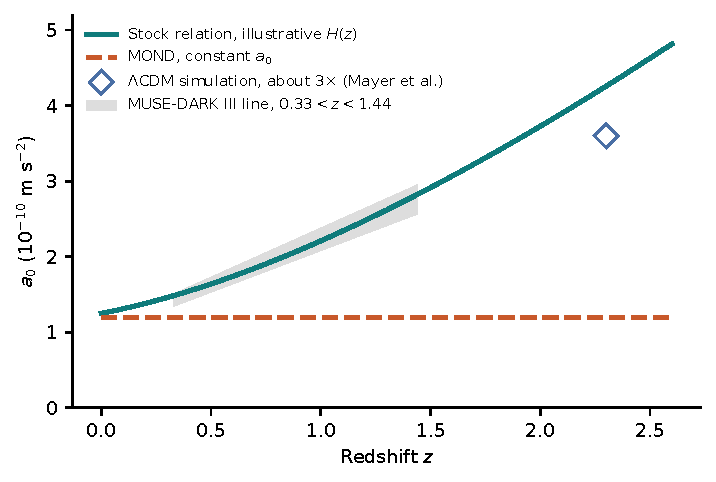
\includegraphics[width=0.72\textwidth]{figures/a0z_three.pdf}
\caption{The acceleration scale against redshift in the three descriptions:
$\epsilon cH(z)$, the constant MOND value, and the approximate rise in
the Magneticum \LCDM\ simulations. The solid curve uses
$H_0=68.42$ and $H/H_0=[0.3038(1+z)^3+0.6962]^{1/2}$, a
matter-plus-constant-vacuum illustration at the frozen fit's present-day
parameters. The gray envelope shifts both MUSE-DARK III Appendix E line
coefficients by their marginal errors over $0.33<z<1.44$; a joint
confidence region requires their covariance.}
\label{fig:a0three}
\end{figure}

\subsection{Why the fitted intercept lies below the local value}

The numerical curve in equation~\eqref{eq:aznumeric} has
$a_0(0)=1.230729\,\aunit$ and $a_0(1)=2.203315\,\aunit$.
The intercept of a line fitted over a positive-redshift interval is a
different quantity from the value of the curved function at zero.

For points $(z_i,f_i)$ with equal weights, minimizing
$\sum_i[f_i-(A+Bz_i)]^2$ gives
\begin{equation}
B=\frac{\sum_i(z_i-\bar z)(f_i-\bar f)}
{\sum_i(z_i-\bar z)^2},\qquad A=\bar f-B\bar z.
\label{eq:linefit}
\end{equation}
Using $z_i=0.33,0.34,\ldots,1.44$ gives equation~\eqref{eq:projection}.
The resulting intercept is $1.003$ and the slope is $1.226$; both are
within the published marginal errors.

The curvature follows analytically. Write
$u=1+z$ and $E=\sqrt{\Omega_m u^3+\Omega_\Lambda}$. Then
\begin{equation}
\frac{d^2E}{dz^2}
=\frac{3\Omega_m u\,[\Omega_m u^3+4\Omega_\Lambda]}{4E^3}>0.
\end{equation}
Across the stated interval, a single straight line averages the increasing
slope and extrapolates below the true value at $z=0$. The lower intercept
therefore has a direct mathematical explanation within the proposed
curve. Its precise size depends on the interval and weights.

\begin{figure}[htbp]
\centering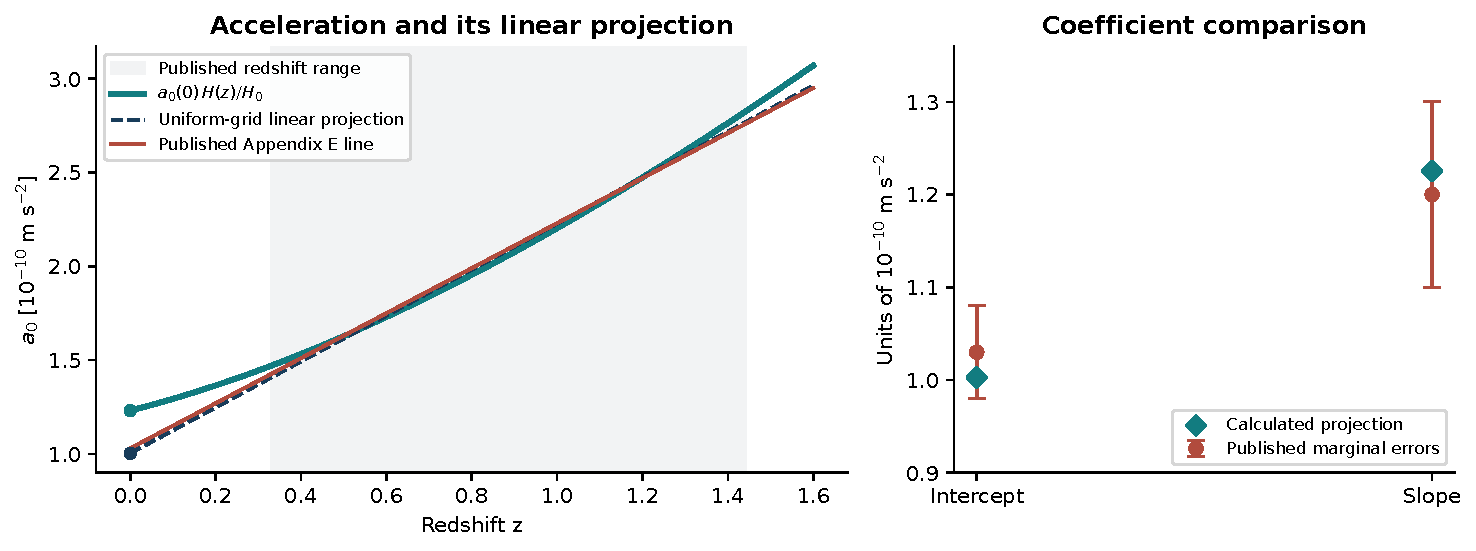
\includegraphics[width=\textwidth]{figures/redshift.pdf}
\caption{The calculated acceleration curve and its linear projection.
The published line summarizes the Appendix E inference. The right panel
shows marginal coefficient errors, with no assumption of independence.
The uniform-grid projection is not a refit to the original galaxy data.}
\end{figure}

The individual coefficient differences are $-0.54$ and $+0.26$ times the
quoted marginal errors. A joint significance requires the fitted
intercept--slope covariance and the survey's effective redshift weighting.
The two agreements are consequences of one curve, not independent
probabilities to multiply.

\subsection{A joint cosmological test}

The prediction fixes the absolute function, including normalization and
curvature. This comparison uses $\Omega_m=0.315$ and
$\Omega_\Lambda=0.685$. A joint test must use the release model's
fitted $H(z)$ in equation~\eqref{eq:a0}, propagate its uncertainty, and
fit the individual galaxies with their correlated baryonic and kinematic
errors. Galaxy formation can also produce an evolving RAR in conventional
halo models, so evolution alone does not distinguish the mechanisms.

\subsection{Galaxy dynamics measures the Hubble constant}
\label{sec:h0galaxies}
The relation $a_0=\epsilon cH_0$ makes galaxy dynamics an independent measurement of the
Hubble constant, $H_0=a_0/\epsilon c$. The frozen fit's $H_0=68.42$
requires $a_0=1.249\times10^{-10}\,\mathrm{m\,s^{-2}}$, and the
Cepheid-calibrated $73.04$ requires $1.334\times10^{-10}\,\mathrm{m\,s^{-2}}$.
Hubble-flow distances carry almost no information on $H_0$ here, because
the inferred $a_0$ scales with the assumed distance scale in nearly the
same way as the prediction. The 44 SPARC galaxies with tip-of-the-red-giant-branch,
Cepheid or supernova distances, fitted with per-galaxy mass-to-light
ratios, distances and inclinations under their priors, give
$a_0=(1.21\pm0.19)\times10^{-10}\,\mathrm{m\,s^{-2}}$, or
$H_0=66\pm11\,\kms\,\mathrm{Mpc}^{-1}$. All 153 galaxies of quality 1--2
give $1.03\pm0.11$, and the subsamples range from $0.97$ for gas-dominated
dwarfs to $1.37$ for massive galaxies with absolute distances; that drift,
also seen in Section~\ref{sec:sparcthree}, sets the present systematic
floor. A $2\%$ determination of $a_0$ with absolute distances separates
$68.4$ from $73$ at $3\sigma$.
\source{T1, section 27.3}


\subsection{A common CMB-to-galaxy normalization}
\label{sec:crossnorm}
The bare commitment ratio and galactic scale obey
\begin{equation}
\left(\frac{\rho_{C,i}}{\rho_{b,i}}\right)_{\rm bare}=\frac1\epsilon,\qquad
a_0(z)=\epsilon cH(z),\qquad
a_0(z)\left(\frac{\rho_{C,i}}{\rho_{b,i}}\right)_{\rm bare}=cH(z).
\end{equation}
The fitted formation convention includes the mass-conversion factor
$f_m=5.333\epsilon$, and release leaves the homogeneous survival factor
$s(z)=e^{-\eta_*F(z)}$. On the undepleted background branch, the
observable stock ratio therefore satisfies
\begin{equation}
a_0(z)\frac{\bar\rho_C(z)}{\bar\rho_b(z)}=f_m s(z)cH(z).
\label{eq:crossnorm}
\end{equation}
The standard linear-depletion configuration gives
$H_0=68.458\,\kms\,\mathrm{Mpc}^{-1}$ and
$a_0(0)=1.25005\times10^{-10}\,\mathrm{m\,s^{-2}}$,
about 1.6\% above the reference value. The exponential-allocation fit with
massless neutrinos, linear lensing and a low-redshift supernova offset gives
$H_0=68.93885586416\,\kms\,\mathrm{Mpc}^{-1}$ and
$a_0(0)=1.25883\times10^{-10}\,\mathrm{m\,s^{-2}}$,
about 2.3\% above the reference value. The frozen four-parameter fit of
Section~\ref{sec:coolinggate} gives $H_0=68.42\,\kms\,\mathrm{Mpc}^{-1}$
and $a_0(0)=1.2494\times10^{-10}\,\mathrm{m\,s^{-2}}$, 1.5\% above the
reference value. Each value follows from its fitted
$H_0$ without a separate fit of $a_0$.
This is a conditional relation between sectors. Cosmological abundance
and $H_0$ are inferred together; galaxy mass calibration limits the
elementary empirical comparison to roughly twenty percent. The tilt-mode pendulum length and mass convention retain their physical matching assumptions.
\source{U1, S02; T4--T5}

\subsection{Newton's constant and charged-lepton masses}
\label{sec:constants}
The selected particle-coefficient route gives
$G_*=6.6742890813\times10^{-11}\,\mathrm{m^3\,kg^{-1}\,s^{-2}}$,
$-0.073$ quoted CODATA standard deviations; the muon ratio is
$206.768280237$, at $-0.535$ quoted standard deviations. Its tau mass
is 1776.9188 MeV against $1776.93\pm0.09$ MeV. Of the 401 tested
routing integers, only the integer $7$ lies within two quoted standard deviations
for the stated route; of 43 tested Farey candidates, only $2/7$ lies
within one. These finite-menu uniqueness checks do not quantify the
historical search over possible formulas. The measured Newton scale
and marked-formula residuals were known during development. An independent
muon measurement with one tenth of the current uncertainty and the same
central value would lie $5.35\sigma$ above the selected ratio. The tau
mass tests the additional second-shell factor. \source{T1, section 27.4}
\source{U1, S11}\cite{constantsnew}

\subsection{Wide binaries and Solar-System null tests}
\label{sec:binaries}
With the parent-carrier rule, a wide binary has no independent capacity
halo. A radial Galactic-tide estimate for one to two solar masses at
10--30 kAU gives $\Delta v/v\simeq1.1\times10^{-5}$--$6\times10^{-4}$.
The range depends on separation, mass, and orientation; a universal
$10^{-4}$ ceiling is unwarranted. The selected Solar quadrupole
$Q_2=0$ is 0.89 quoted standard deviations from the Cassini central
value. No full Gaia selection-and-contamination likelihood has been
performed. \source{U1, S10}

MOND with the Galactic external field predicts relative velocities about
20\% above the Newtonian value at separations beyond a few kAU. Analyses
of Gaia DR3 disagree: Chae reports a low-acceleration boost, and Banik et
al. find a strong preference for Newtonian gravity. The stock prediction coincides with general relativity
and \LCDM, so a settled wide-binary result separates the stock model from
MOND. \cite{chae23,banik24}

\subsection{Stock selection discriminants}
\label{sec:stocklags}
For a fixed baryonic field, a delay $\tau$ makes the fitted acceleration
scale sample $\epsilon cH(t-\tau)$. At $z=0.97$ the MOND-based fit of
Section~\ref{sec:redshift} then gives $\tau<0.66\,$Gyr at $95\%$
confidence. Evolution of the baryonic field also shifts the fitted scale.
\cite{ciocan} \source{T1, section 15}

In a spherical Milky Way model with fixed baryons, eight realizations of
$4000$ stock particles settled for $10\,$Gyr at the $z=2$ scale with one
contact proposal per orbit and then followed $a_0=\epsilon cH(t)$. At
$z=0.97$ the fitted scale differed from its fixed-scale value by $0.4\%$,
$-0.1\%$, $-1.1\%$ and $0.5\%$ at $10$, $20$, $30$ and $50\,$kpc, with
standard errors near $1\%$. The observational limit corresponds to an
excess of $11\%$. A step in $a_0$ from the $z=0.97$ value to its present
value, measured against a paired run at unchanged scale, reached
$1-e^{-1}$ of the change after $0.25$, $0.38$ and $0.49\,$Gyr at $5$,
$10$ and $20\,$kpc at one proposal per orbit, and after $0.12$, $0.14$
and $0.24\,$Gyr at three. These step times exceed the lag of the gradual
change. \source{T1, O.3; G13}

The selection gives the following tests.
\begin{itemize}
\item for a fixed baryonic target and $a_0$, relaxation reduces residuals
from the response law with time since the last major accretion; longer
outer orbits can retain larger residuals at a given age. Evolution of the
target adds a history-dependent lag;
\item at $z\simeq1$ the model predicts an outward rise of the acceleration
scale inferred from the stock, beyond a radius set by the contact rate. In
the same runs the excess over the fixed-scale value at $z=0.97$ was $9\%$
at $100\,$kpc and $30\%$ at $200\,$kpc, with standard errors of $1\%$ and
$2\%$. The runs start from a settled state at $z=2$, which makes these
lower estimates. Radial mass profiles at intermediate redshift can test
the predicted rise. \source{T1, O.3; G13}
\item isolated ellipticals follow the law out to the radius where their hot
gas outweighs their stars;
\item the ratio $a_0(z)/a_0(0)=H(z)/H_0$ applies to relaxed systems, and a
$3\sigma$ distinction from a conventional rise of about three at $z=2.3$
\cite{mayer22} needs a total uncertainty near 4.5\%.
\end{itemize}
The dwarf runs reach the law at the mass of rotationally supported dwarfs.
The GravSphere sample at $10^4<M_{\rm bar}/\Msun<10^{7.5}$ lies above the
extrapolated relation \cite{julio25}, and the selection does not yet
extend to that regime.
\source{G8, G9}

